%% Charlie Redmon
%% 20170914
%% Game theory tree diagram example

\documentclass[border=15pt]{standalone}

%% Charlie Redmon
%% 20170911
%% setupGameTheoryStyle.tex: style configurations for game theory


\usepackage{tikz}
\usetikzlibrary{patterns}
\usetikzlibrary{calc}

% Specify spacing for each level of the tree
\tikzstyle{level 1}=[level distance=15mm,sibling distance=25mm]
\tikzstyle{level 2}=[level distance=15mm,sibling distance=15mm]

\tikzset{
	% Two node styles for game trees: solid and hollow
	solid node/.style={circle,draw,inner sep=1.5,fill=black},
	hollow node/.style={circle,draw,inner sep=1.5}
}


\begin{document}

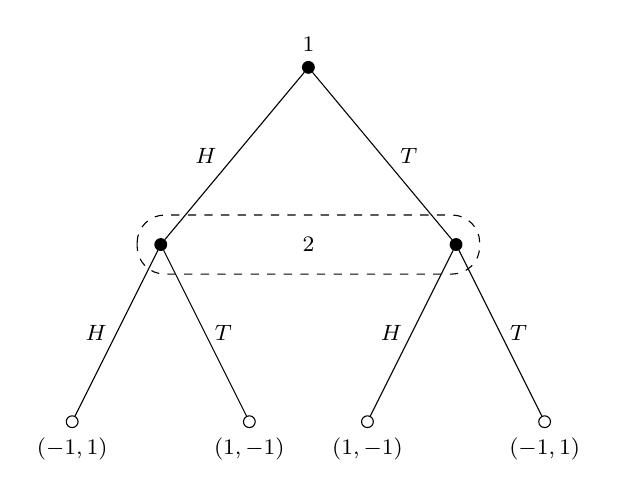
\begin{tikzpicture}[scale=1.5,font=\footnotesize]

% set top (root) node (level 1)
\node(0)[solid node,label=above:{$1$}]{}
	% child L
	child{node(1)[solid node]{}
      % child L.L
      child{node[hollow node,label=below:{$(-1,1)$}]{} edge from parent node[left]{$H$}}
      % child L.R
      child{node[hollow node,label=below:{$(1,-1)$}]{} edge from parent node[right]{$T$}}
      edge from parent node[left,xshift=-3]{$H$}
	}
    % child R
	child{node(2)[solid node]{}
      % child R.L
      child{node[hollow node,label=below:{$(1,-1)$}]{} edge from parent node[left]{$H$}}
      % child R.R
      child{node[hollow node,label=below:{$(-1,1)$}]{} edge from parent node[right]{$T$}}
      edge from parent node[right,xshift=3]{$T$}
	};
	% information set (rounded dashed-line rectangle)
	\draw[dashed,rounded corners=10]($(1) + (-.2,.25)$)rectangle($(2) +(.2,-.25)$);
	% specify mover at 2nd information set
	\node at ($(1)!.5!(2)$) {$2$};

\end{tikzpicture}

\end{document}